\documentclass[12pt,a4paper]{article}

% 使用中文宏包
\usepackage[UTF8]{ctex}
\usepackage{authblk}
\usepackage{graphicx} %插入图片的宏包
\usepackage{float} %设置图片浮动位置的宏包
\usepackage[strings]{underscore}
\usepackage{times}
\usepackage{epsfig}
\usepackage{amsmath}
\usepackage{amssymb}
\usepackage{overpic}
\usepackage{listings}
\usepackage{color}
\usepackage{enumitem}
\setenumerate[1]{itemsep=0pt,partopsep=0pt,parsep=\parskip,topsep=5pt}
\setitemize[1]{itemsep=0pt,partopsep=0pt,parsep=\parskip,topsep=5pt}
\setdescription{itemsep=0pt,partopsep=0pt,parsep=\parskip,topsep=5pt}

\definecolor{mygreen}{rgb}{0,0.6,0}
\definecolor{mygray}{rgb}{0.5,0.5,0.5}
\definecolor{mymauve}{rgb}{0.58,0,0.82}
\lstset{ %
  backgroundcolor=\color{white},   % choose the background color
  basicstyle=\footnotesize,        % size of fonts used for the code
  breaklines=true,                 % automatic line breaking only at whitespace
  captionpos=b,                    % sets the caption-position to bottom
  commentstyle=\color{mygreen},    % comment style
  escapeinside={\%*}{*)},          % if you want to add LaTeX within your code
  keywordstyle=\color{blue},       % keyword style
  stringstyle=\color{mymauve},     % string literal style
}

\usepackage[pagebackref=true,breaklinks=true,letterpaper=true,colorlinks,bookmarks=false]{hyperref}


\def\httilde{\mbox{\tt\raisebox{-.5ex}{\symbol{126}}}}


\graphicspath{{figures/}}

\setcounter{page}{1}

\begin{document}


%%%%%%%%% TITLE

\title{奇异值分解在卷积神经网络中的应用}
\author[*]{纳文琪}
\date{}
\affil[*]{信息学院,学号:22018000164}
\maketitle


\section{引言}
\paragraph{} 人工神经网络(Artificial Neural Networks, ANN)是上世纪80年代以来的研究热点,主要以模拟人脑神经细胞的方式,ANN分别以卷积神经网络(Convolutional Neural Networks, CNN)和循环神经网络(Recurrent Neural Netowrks, RNN)两种方式在自然语言处理、图像处理方面得到了广泛应用。自问世以来,由于受计算能力的限制,ANN并未得到大规模的应用。直到本世纪初,得益于计算能力提升,特别是GPU在大规模矩阵运算和反向传播算法中的应用,ANN得到了快速发展。特别在图像识别领域,2012年AlexNet\cite{alexnet} 利用CNN实现的图像分类方法在多个分类竞赛中夺得了冠军,2015年ResNet\cite{resnet} 网络的图像识别错误率已经低于人类。
\paragraph{} CNN虽然可以有效地解决一些图像处理的问题,然而,由于CNN网络一般较大,导致参数太多。例如,VGG16\cite{vgg} 网络的参数已经达到了1.3亿个。参数太多最终将导致两个主要问题:首先是网络训练效率低,特别是当训练数据维度太大,例如大分辨率的图片时,网络训练效率会很低,甚至可能出现内存溢出的情况;其次是容易引起过拟合问题,当网络参数的数量远远多于数据集数量时尤为明显。因此,如何减少CNN的参数是一个值得研究的议题。
\paragraph{} 为了减少CNN中的参数,一定程度上提高训练效率,我们在本文中提出一种降低卷积神经网络参数的方法:在将图像送入卷积神经网络之前,先将图片进行奇异值分解,选取合适的秩,降低输入数据的维度,从而减少网络参数。
\paragraph{} 奇异值分解(Singular Value Decomposition, SVD)是线性代数中一种常用的特征分解方法。具体表示为:
\begin{equation}
	M=U\Sigma V^T
\end{equation}
它可以将一个较大的矩阵$M$转换成两个较小的矩阵$U$、$V$和一个对角矩$\Sigma$来表示。因为通常情况下$M$的维度比较大,而分解后的矩阵可以通过调整$\Sigma$的秩来调节大小,因此我们常常通过调整$\Sigma$的秩的大小来得到一个原矩阵的近似表示,而此近似表示通常所占空间比原矩阵小得多。奇异值分解会使原矩阵数据有一定的损失,但一般来讲损失较小,只需取10\%的秩即可获得原矩阵大约99\%的数据。SVD方法常常被用于图像压缩、推荐系统等方面。
\paragraph{} 卷积神经网络中减少网络参数的做法通常是:使用卷积操作代替全联接或使用Patch的方法\cite{pix2pix} 代替整个图片的卷积。我们考虑到通过奇异值分解后得到的$U$、$V$和$\Sigma$也是原图像的一种表示,且包含相对较全的信息。CNN中参数的数量由网络结构和网络的输入决定,当网络结构固定时,如果能够以另外一种输入参数更少的表示输入的图像的话,将会使网络参数减少。因此,我们考虑先将大图片进行奇异值分解,再将分解的结果输入卷积神经网络中进行计算。

\section{方法}
\paragraph{} 在这个部分,我们在卷积神经网络引入奇异值分解方法,以达到减少网络参数的目的。如图 \ref{Fig.model}所示,我们将引入SVD的卷积神经网络计算分为3个步骤。
\begin{figure}[H]
		\centering
		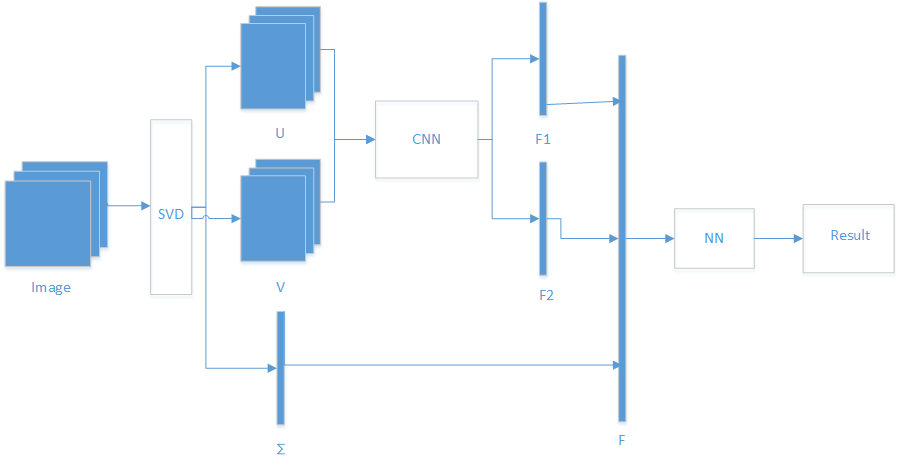
\includegraphics[width=0.7\textwidth]{../images/svd-cnn-arch.png}
		\caption{引入SVD的卷积神经网络}
		\label{Fig.model}
	\end{figure}
	
	\subparagraph{} 首先,我们假定输入的图片的维度为$h\times w$,即图片高为$h$,宽为$w$,且只有一个通道。在将图片输入到卷积神经网络之前,我们先对图片进行奇异值分解,得到的$U$、$V$、$\Sigma$的维度分别是:$h\times r$,$w \times r$,$r\times 1$,其中,$r \ll h$且$r \ll w$。
	\subparagraph{} 随后,我们将U和V输入到预先定义好的卷积神经网络中,并通过卷积层和扁平化层得到两个向量$F_1$和$F_2$。
	\subparagraph{} 最后,将$F_1$、$F_2$和$\Sigma$叠加在一起,组成一个向量$F$,再将F输入到卷积神经网络最后的全连接层中即可得到输出。
\paragraph{} 通过以上方式,可将一个大的矩阵分解输入为两个小的矩阵和一个向量的输入,通过调整$r$的值可以控制网络所需的参数的数量。


\section{局限}
\paragraph{} 以上所提的方法目前还处于试验阶段,但由其原理及前期所做的测试不难看出,将奇异值分解方法以这样的方式应用到卷积神经网络中将可能会遇到两个问题。首先,对矩阵进行奇异值分解本身是需要消耗计算资源的,这方面可能会导致计算效率降低,运算时间变长。但是,由于卷积神经网络的训练往往会将数据集输入到网络中多次,如果我们将第一次进行奇异值分解的结果保存下来,那么下一次输入卷积神经网络的时候就没有必要再进行奇异值分解了。因此,当训练输入轮次较多时,我们可以认为在整个训练过程中奇异值分解运算的时间复杂度为常数,对训练效率影响不大。其次,经前期实验发现,矩阵经奇异值分解后的结果将原来的方阵变换成了行列树不等的矩阵,这样的矩阵会限制卷积运算的次数,从而导致输入到全连接层的参数变多,最终使得整个网络的参数没有减少,反而增多。为了解决这个问题,我们需要针对网络的卷积层设置不同的卷积核大小,以便卷积结果可以收敛为更小的矩阵。
\paragraph{} 接下来的工作中,我们将继续进行相关实验,以验证将奇异值分解引入卷积神经网络网络的方法是否可行,是否可以在一定程度上提高训练效率。与此同时,还需要考虑提高训练效率的同时,是否会对卷积神经网络的分类精度带来损失。





\bibliographystyle{ieeepes}
\bibliography{../Saliency}
\end{document}



























































